%Chapter 2
\chapter{Preliminare}%informatii despre teoria limbajelor formale -pe scurt info despre automate finite si metode de transformare a gramaticilor
\label{Chapter2}
\lhead{Capitolul 2. \emph{Preliminare}}
\begin{quotation}


 Fie T o mul\c time de simboluri denumit\v a alfabet. Orice submul\c time a mul\c timii $T^{*}$ reprezint\v a un limbaj asupra alfabetului T. Elementele limbajului se numesc propozi\c tii. Dac\v a limbajul este finit atunci el poate s\v a fie definit prin enumerare. De exemplu consider\^ and alfabetul B = $\lbrace$ 0, 1 $\rbrace$ atunci L = $\lbrace$01, 10, 101 $\rbrace$ este un limbaj. Mul\c timea cuvintelor din limbajul natural este \c si el un limbaj pentru care se poate pune problema enumer\v arii tuturor cuvintelor, chiar dac\v a lista care ar rezulta este imens\v a, deci este un limbaj reprezentabil prin enumerare. Dar cazul interesant este cel \^n care limbajul este infinit. S\v a consider\v am de
exemplu limbajul "\c sirurilor formate din 0 \c si 1 a c\v aror lungime este divizibil\v a cu 3". Evident este vorba de un limbaj infinit. Textul prin care am specificat limbajul constituie o reprezentare finit\v a a limbajului. Nu este singura solu\c tie posibil\v a de reprezentare finit\v a. De exemplu dac\v a notam cu L limbajul respectiv atunci:  
$$ L = \lbrace w \in \lbrace0,1 \rbrace^{*} \slash |w| mod 3 = 0 \rbrace$$
este un alt mod de a specifica acela\c si limbaj. 
\end{quotation}
\begin{quotation}
 \^ In general exist\v a doua mecanisme distincte de definire finit\v a a limbajelor: prin generare sau prin recunoa\c stere. \^In primul caz este vorba de un "dispozitiv" care \c stie s\v a genereze toate propozi\c tiile din limbaj (\c si numai pe acestea) astfel \^inc\^ at aleg\^ and orice propozi\c tie din limbaj \^ intr-un interval finit de timp dispozitivul va ajunge să genereze propozi\c tia respectiv\v a. \^ In al doilea caz este vorba de un "dispozitiv" care \c stie s\v a recunoasc\v a (s\v a accepte ca fiind corecte) propozi\c tiile limbajului dat. 
\end{quotation}

\section{Gramatici}
\begin{quotation}
%O gramatica Chomsky este o constructie: G=(N,T,P,S) unde: N=multimea finita de neterminali,T=multime %finita de "terminali" :$N\cap T=\emptyset,S\in N $=este simbolul de "start" si $P\subseteq(N\cup %T)^{*}N(N\cup T)^{*}\times(N\cup T)^{*}$ este o multime finita de productii.
 O gramatic\v a reprezint\v a cel mai important exemplu de generator de limbaje. Prin defini\c tie o gramatic\v a este G = (N, T, P, S) unde :
 \begin{itemize}
 \item {N este o mulţime finită de simboli numită mulţimea simbolilor neterminali;}
 \item {T este o mul\c time finit\v a de simboli numit\v a mul\c timea simbolilor terminali,($N\cap T=\emptyset$);}
 \item {P este o submul\c time finit\v a din $(N\cup T)^{*}N(N\cup T)^{*}\times(N\cup T)^{*} $;numit\v a mul\c timea produc\c tiilor gramaticii. Un element $(\alpha,\beta)\in P$ este notat cu $\alpha \rightarrow \beta$ \c si se nume\c ste produc\c tie.  
 }
 \item {$S \in N $ este un simbol special numit simbol de start al gramaticii G.}

\end{itemize}  
\end{quotation}
\subsection{Transform\v ari asupra gramaticilor independente de context}
\begin{quotation}
Din punctul de vedere al procesului de compilare, gramaticile sunt utilizate pentru faza de analiz\v a 
sintactic\v a, pentru care se utilizeaz\v a gramatici independente de context. Exist\v a o serie de metode de analiza sintactic\v a, bine puse la punct at\^ at din punct de vedere teoretic c\^ at şi practic. Fiecare dintre aceste metode impune \^ins\v a o serie de restric\c tii asupra gramaticilor utilizate. \^In general atunci c\^ and se construie\c ste o gramatic\v a se pleac\v a de la forma general\v a a structurilor pe care aceasta trebuie s\v a le descrie \c si nu de la metoda de analiz\v a sintactic\v a ce va fi utilizat\v a. \^In acest mod se ob\c tine o gramatic\v a ce poate să fie "citit\v a" u\c sor de c\v atre proiectant. Pentru a satisface \^ ins\v a condi\c tiile impuse de c\v atre metodele de analiz\v a sintactic\v a sau de c\v atre generarea de cod, se realizeaz\v a transform\v ari asupra gramaticilor. Aceste transform\v ari trebuie s\v a p\v astreze neschimbat limbajul generat. \^In cele ce urmeaz\v a vom prezenta c\^ ateva transform\v ari tipice asupra gramaticilor independente de context. Pentru a explica semnifica\c tia acestor transform\v ari \^ in contextul analizei sintactice vom prezenta \^ int\^ ai no\c tiunea de arbore de derivare. 
\end{quotation}
\begin{quotation}
 Un arbore de derivare este o reprezentare grafic\v a pentru o secven\c t\v a de deriv\v ari (de aplic\v ari ale rela\c tiei $\Rightarrow$ \^ intre formele propozi\c tionale). \^ Intr-un arbore de derivare nu se mai poate identifica ordinea \^ in care s-a  f\v acut substitu\c tia simbolilor neterminali. Fiecare nod interior arborelui, reprezint\v a un neterminal.Descenden\c tii unui nod etichetat cu un neterminal A sunt eticheta\c ti de la st\^ anga la dreapta prin simbolii care formeaz\v a partea dreapt\v a a unei produc\c tii care are \^ in partea st\^ anga neterminalul A. Parcurg\^ and de la st\^ anga la dreapta frunzele unui astfel de arbore se ob\c tine o form\v a propozi\c tional\v a. S\v a consider\v am de exemplu din nou gramatica \c sirurilor de paranteze bine formate:\\
$  G = (\lbrace S \rbrace, \lbrace(,)\rbrace, \lbrace S → (S)S \vert \lambda \rbrace, S)$ \\
Fie urm\v atoarea secven\c t\v a de deriv\v ari:\\
$ S \Rightarrow ( S ) S \Rightarrow ( ( S ) S ) S \Rightarrow ( () S ) S \Rightarrow 
 ( () ( S ) S ) S \Rightarrow ( () () S ) S \Rightarrow 
 ( () () ) S \Rightarrow ( () () ) ( S ) S \Rightarrow^{*}( ()() ) ()$\\
 Se ob\c tine arborele de derivare:\\
 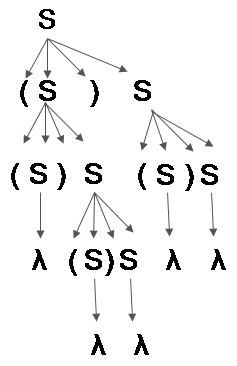
\includegraphics{arbore1.png}
 \label{arbore1}
\end{quotation}
\subsection{Eliminarea ambiguit\v a\c tii}
O gramatic\v a care produce mai mul\c ti arbori de derivare pentru aceea\c si propozi\c tie este o gramatic\v a 
ambigu\v a. Deoarece exist\v a tehnici de analiz\v a sintactic\v a care lucreaz\v a numai cu gramatici neambigue vom \^ incerca s\v a construim gramatici care genereaz\v a acela\c si limbaj \c si care sunt neambigue.  S\v a consider\v am de exemplu urm\v atoarea gramatic\v a: 
\begin{verbatim}
instr → if expresie then instr | 
 if expresie then instr else instr |
 alte_instr 
\end{verbatim}
S\v a construim arborele de derivare pentru propozi\c tia : 
\begin{verbatim}
if E1 then if E2 then S1 else S2
\end{verbatim}

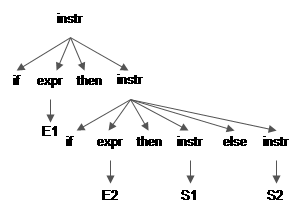
\includegraphics[scale=1]{arbore2.png}
\\
Pentru aceast\v a propozi\c tie mai exist\v a \^ins\v a un arbore de derivare.
\\
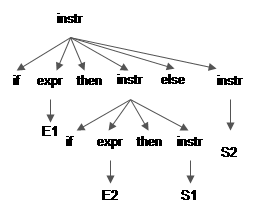
\includegraphics[scale=1]{arbore3.png}

\paragraph*{}
\^In toate limbajele de programare care accept\v a construc\c tii de tip if then else se consider\v a cu sens prima derivare \^ in care fiecare clauza else este atribuit\v a instruc\c tiunii if cea mai interioar\v a. Rezult\v a deci condi\c tia pe care trebuie s\v a o satisfac\v a o instruc\c tiune if. Instruc\c tiunea cuprins\v a \^ intre then \c si else trebuie s\v a nu fie o instruc\c tiune if sau s\v a fie o instruc\c tiune if cu clauza else. Rezult\v a urm\v atoarea gramatic\v a ob\c tinut\v a prin
transformarea gramaticii anterioare: 
\begin{verbatim}
instr → if_cu_else| if_fara_else                               
  if_cu_else → if expresie then if_cu_else else if_cu_else |      
                alte_instr                                        
  if_fara_else → if expresie then instr |                         
                  if expresie then if_cu_else else if_fara_else 
\end{verbatim}

Se observ\v a c\v a aceast\v a gramatic\v a genereaz\v a acela\c si limbaj cu gramatica anterioar\v a dar accept\v a o derivare unic\v a pentru propozi\c tia : 
\begin{verbatim}
 if E1 then if E2 then S1 else S2 
\end{verbatim}
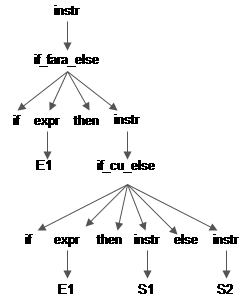
\includegraphics[scale=1]{arbore4.png}
\paragraph*{}
Se nume\c ste produc\c tie ambigu\v a o produc\c tie care are \^ in partea dreapt\v a mai multe apari\c tii ale aceluia\c si simbol neterminal.Existen\c ta unei produc\c tii ambigue nu implic\v a faptul că gramatica este ambigu\v a.
%______________________________________
%
%
%
%
%_______________________________________
\subsection{Eliminarea recursivit\v a\c tii st\^ anga }
\paragraph*{}
O gramatic\v a este recursiv\v a st\^ anga dac\v a exist\v a un neterminal A astfel \^ inc\^ at exist\v a o derivare A $\Rightarrow ^{*}$ A$\beta$
pentru $\beta \in(T \cup N)^{*}$. O analiz\v a sintactic\v a descendent\v a determinist\v a nu poate s\v a opereze cu o astfel de gramatic\v a, deci este necesar\v a o transformare.
S\v a consider\v am \^ int\^ ai cazul cel mai simplu pentru care \^ in
gramatic\v a exist\v a produc\c tii de forma $A \rightarrow A\beta | \alpha$. \^In acest caz limbajul generat este de forma $\alpha \beta$ cu n ≥ 0.
Acela\c si limbaj poate s\^ a fie generat de c\v atre gramatica: A → $\alpha$A', A' → $\beta$A'| $\lambda$. 
\\
 S\v a consider\v am de exemplu gramatica expresiilor aritmetice :\\
 $ E \rightarrow E + T | T, T \rightarrow T * F | F, F \rightarrow (E) | a $
\\
 Se observ\v a ca pentru un \c sir de forma a+a*a,examinand numai primul simbol terminal (a) nu este clar cu ce produc\c tie dintre produc\c tiile pentru E trebuie s\v a se \^inceap\v a derivarea.Aplic\^ and ideea anterioar\v a se ob\c tine:\\
$ E \rightarrow T E', E' \rightarrow +TE' | \lambda, T \rightarrow FT', T' \rightarrow *FT' | \lambda, F \rightarrow (E) | a $
\\
\^In acest caz derivarea va \^incepe sigur prin aplicarea produc\c tiei Ε → TE' \c si se ob\c tine derivarea Ε $\Rightarrow$ TE' $\Rightarrow$ FT'Ε'. \^In acest moment se vede c\v a pentru F trebuie s\v a se aplice produc\c tia F $\rightarrow$ a. Deci se ob\v tine Ε $\Rightarrow$ aT'Ε'. Urmeaz\v a simbolul terminal + datorit\v a c\v aruia pentru T' se va aplica produc\c tia T' → $\lambda$, etc. 
\paragraph*{}
Dac\v a gramatica nu permite deriv\v ari de tipul A $\Rightarrow ^{*}$ A (f\v ar\v a cicluri ) \c si nu con\c tine $\lambda$ - produc\c tii poate s\v a fie transformat\v a \^ in vederea elimin\v arii recursivit\v a\c tii st\^ anga utiliz\^ and urm\v atorul algoritm, ob\b tin\^ andu-se o gramatic\v a echivalent\v a f\v ar\v a recursivitate st\^ anga. 

\textit{
Se aranjeaz\v a neterminalele \^ in ordinea A1, ..., An\\
pentru i = 1 p\^ an\v a la n  executa \\
pentru j = 1 p\^ an\v a la i - 1 executa \\ 
\^inlocuie\c ste fiecare produc\c tie de forma $A_{i} \rightarrow A_{j} \beta$ cu produc\c tiile \\ $A_{i} \rightarrow → \alpha_{1}\beta | \alpha_{2}\beta|...|\alpha_{k}\beta  $ \\
unde $A_{j}\rightarrow \alpha_{1}|\alpha_{2}|\alpha_{3}|...|\alpha_{k}$\\
sunt toate produc\c tiile pentru $A_{j}$
\\
elimin\v a recursivitatea st\^ ang\v a \^ intre produc\c tiile $A_{i}$
}


%________________________________


\subsection{Factorizare st\^ anga}
\paragraph*{}
 Acest tip de transformare este util pentru producerea unei gramatici potrivite pentru analiza sintactic\v a 
descendent\v a de tip determinist. Ideea este că dac\v a nu este clar care dintre produc\c tiile alternative poate s\v a fie aplicat\v a pentru un neterminal se va am\^ ana luarea unei decizii p\^ an\v a c\^ and s-a parcurs suficient din \c sirul
de intrare pentru a se putea lua o decizie. S\v a consider\v am de exemplu produc\c tiile : \\
S $\rightarrow$ AbS $|$A \\
A $\rightarrow$ BcA $|$B \\
B $\rightarrow$ a $|$ dSd 
\paragraph*{}

S\v a presupunem c\v a \^ incerc\v am s\v a construim \c sirul deriv\v arilor pentru a b a c a pornind de la simbolul de start al gramaticii. Din recunoa\c sterea simbolului a la \^ inceputul \c sirului nu se poate \^ inc\v a trage concluzia care dintre cele doua produc\c tii corespunz\v atoare neterminalului S trebuie s\v a fie luata \^ in considerare (abia la \^ int\^ alnirea caracterului b pe \c sirul de intrare se poate face o alegere corect\v a). \^In general pentru produc\c tia $A \rightarrow \alpha \beta_{1} | \alpha \beta_{2}$ dac\v a se recunoa\c ste la intrare un \c sir nevid derivat din $\alpha$ nu se poate \c stii dac\v a trebuie aleas\v a prima sau a doua produc\c tie. Corespunz\v ator este util\v a transformarea: A $\rightarrow \alpha$ A', A'$\rightarrow \beta_{1}|\beta_{2}$. \\
 Algoritmul de factorizare func\c tioneaz\v a \^ in modul urm\v ator. Pentru fiecare neterminal A se caut\v a cel mai lung prefix $\alpha$ comun pentru dou\v a sau mai multe dintre produc\c tiile corespunz\v atoare neterminalului A. Dac\v a $\alpha\neq \lambda $ atunci se \^ inlocuiesc produc\c tiile de forma $A \rightarrow \alpha \beta_{1}$|$ \alpha \beta_{2}$| ... | $\alpha \beta_{n}$| $\delta$ (unde $\delta$ reprezint\v a alternativele care nu \^ incep cu $\alpha$) cu : \\
A $\rightarrow \alpha A' \delta$
A' $\rightarrow \beta_{1}|\beta_{2}|...|\beta_{n}$
A' este un nou neterminal. Se aplic\v a \^ in mod repetat aceast\v a transformare p\^ an\v a c\^ and nu mai exist\v a dou\v a alternative produc\c tii cu un prefix comun pentru acela\c si simbol neterminal.
 Relu\^ and exemplul considerat se ob\c tine :\\
      S $\rightarrow$ AX \\
     X $\rightarrow$ bS $|$ $\lambda$\\
     A $\rightarrow$ BY \\
     Y $\rightarrow$ cA $|$ $\lambda$\\
      B $\rightarrow$ a $|$ dSd \\

Deci \^ in analiza \c sirului a b a la \^int\^ alnirea simbolului b pentru neterminalul Y se va utiliza produc\c tia Y $\rightarrow$ $\lambda$, \^ in acest mod rezult\v a \c sirul de deriv\v ari :\\
   S $\Rightarrow$ AX $\Rightarrow$ BYX  $\Rightarrow$ aYX $\Rightarrow$ ... 
 

%________________________________________________________________________
%SECTIUNEA A DOUA ATOMATE FINITE
%________________________________________________________________________

\section{Automate finite}

Un automat finit este sistemul A=(Q,$\Sigma$,$\delta$,$q_{0}$,F) unde Q si F sunt nul\c timi,nevide, numite mul\c timea starilor respectiv \textit{ alfabetul de intrare}, $q_{0} \in Q $
este \textit{starea initiala},F$\subseteq$Q este \textit{multimea starilor finale} iar
$\delta$ este o func\c tie $\delta : Q x (\Sigma \cup {\varepsilon}) \rightarrow 2^{Q}$,
numita \textit{func\c tia de tranzi\c tie}
(unde prin $2^{Q}$ s-a notat mul\c timea par\c tilor lui Q).
\paragraph*{}
Modelul prezentat mai sus este cel cunoscut in literatura \c si sub denumirea de automat nedeterminist cu $\varepsilon$ - tranzi\c tii.
%adaug definitia automatului finit determinist
Un automat finit poate fi reprezentat prin \textit{tabela de tranzi\c tie} (func\c tia $\delta$) sau prin \textit{graful de tranzi\c tie}
\^In reprezentarea grafului de tranzi\c tie facem conven\c tia ca starile care nu sunt finale sa le reprezent\v am prin cercuri iar cele finale prin p\v atrate.De asemenea $\varepsilon$ -tranzi\c tiile sunt reprezentate prin arce neetichetate.
\textbf{Exemple de automate}\\
Fie Q=\{0,1,2 \} $\Sigma$ =\{a,b,c \} F=\{2\},$q_{0}$=0,iar $\delta$ este dat\v a astfel:

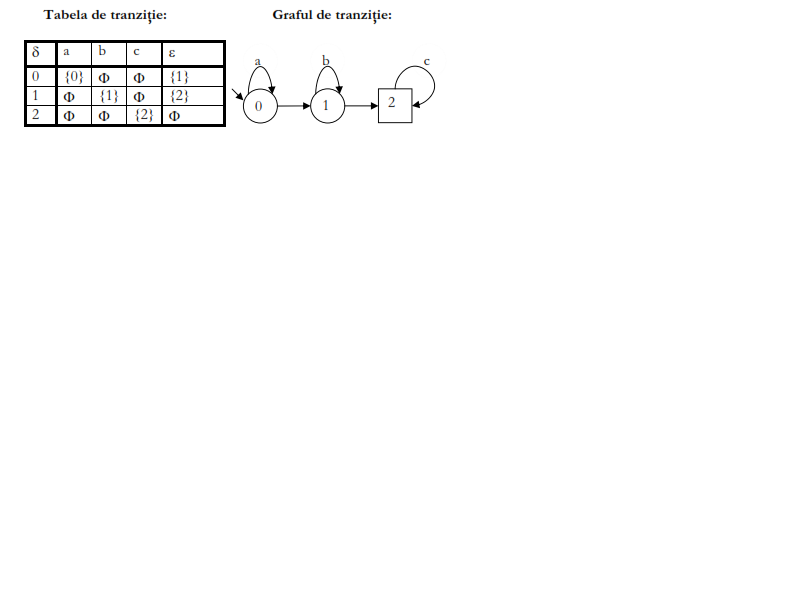
\includegraphics[scale=1]{exemplu_automat.png}


Fie Q=\{0,1,2 \},$\Sigma$=\{a,b \},
F=\{2 \},$q_{0}$=0,iar $\delta$ este:

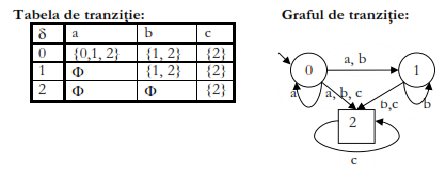
\includegraphics[scale=1]{exemplu_automat2.png}

\textbf{Definitie} Un automat A=(Q,$\Sigma$,$\delta$,$q_{0}$,F) se numeste:
\begin{enumerate}


\item{\textit{nedeterminist} (fara $\varepsilon$ - tranzitii),daca $\delta(q,\varepsilon)=\emptyset$,$\forall q \in Q$}
\item{\textit{determinist},dac\v a
$\delta(q,\varepsilon)=\emptyset$,$\forall q \in Q $ \c si $|\delta(q,a)|\leq 1$ , $\forall q \in Q$,$\forall a \in \Sigma$ 
 } 
\end{enumerate}
%______________________________________
% EXPRESII REGULATE
%______________________________________

\section{Expresii regulate}
Fie $\Sigma$ un alfabet, simbolurile $\varepsilon,\emptyset,|,\bullet,*,),($ care nu apar\c tin lui $\Sigma$ \c si E un cuv\^ ant peste alfabetul $\Sigma \cup \{\varepsilon,\emptyset,|,\bullet,*,),( \}$.O expresie regulat\v a peste $\Sigma$ se define\c ste inductiv astfel: \\
\begin{enumerate}
\item {
E este un \textit{atom regulat} peste $\Sigma$ daca E este un simbol $\Sigma \cup \{ \varepsilon,\emptyset \}$ sau este de forma ($E_{1}$) unde $E_{1}$ este o expresie regulata peste $\Sigma$;
}
\item{E este \textit{factor regulat} peste $\Sigma$ daca E este un atom regulat peste peste $\Sigma$ sau este de forma E1* unde $E_{1}$ este un factor regulat peste $\Sigma$}

\item{
E este un \textit{ termen regulat} peste $\Sigma$ dac\v a
E este un factor regulat peste $\Sigma$
sau este de forma $E_{1}\bullet E_{2}$
unde $E_{1}$ este un termen regulat, iar $E_{2}$ este un factor regulat peste $\Sigma$; 
}
\item{
E este o \textit{expresie regulat\v a} peste $\Sigma$ dac\v a E este un termen regulat peste $\Sigma$ sau este de forma $E_{1}| E_{2}$, unde $E_{1}$ este o expresie regulată, iar $E_{2}$ este un termen regulat peste
$\Sigma$. 
}
\end{enumerate}
Aici $\varepsilon,\emptyset$ sunt privite ca simple simboluri f\v ar\v a vreo semnifica\c tie. Mai jos, interpretarea acestor expresii va fi desigur limbajul \{$\varepsilon$ \} respectiv limbajul vid. 
